
\subsection{Relative error as a function of mode}
We can understand why it is so hard to produce good fits by examining the relative error between different fitting techniques as a function of mode. Look at the relative error between the fit method and the median method. One would hope that absolute error decreases with l, such that the infinite series would be convergent. Since the self force over l scales as a power law that goes as $l^{-2}$ to the first order, I suggest a weight that scales as $l^-{2}$. A weighted fit is of the form

\begin{equation}
  \chi^2=\sum\frac{(f(x_i)-y_i)^2}{\sigma_i}
\end{equation}

where $\sigma_i$ is a weight related to the ``error'' or ``uncertainty'', in this case the truncation or roundoff error depending which regime the mode is in. Absolute values of weights don't matter unless the reduced $\chi^2$ is used to select the best fit. 

%\begin{figure}
%  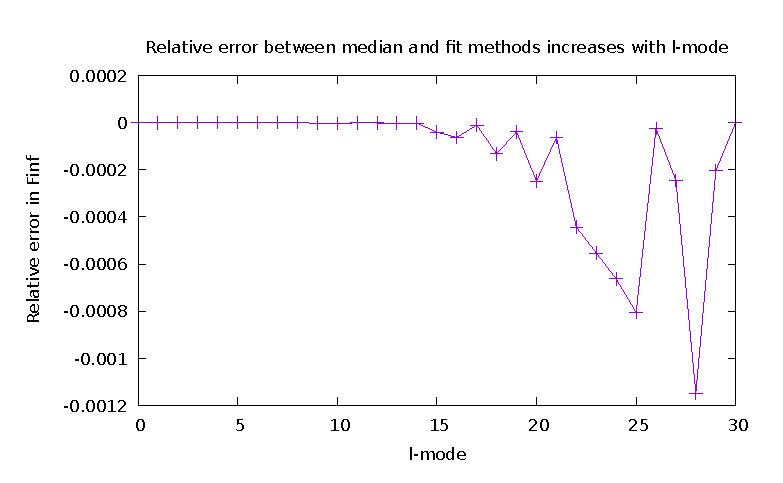
\includegraphics{relErrorIncreaseslMode}
%  \caption{Relative error between fit and median techniques increases with l-mode}
%\end{figure}


\begin{figure}
  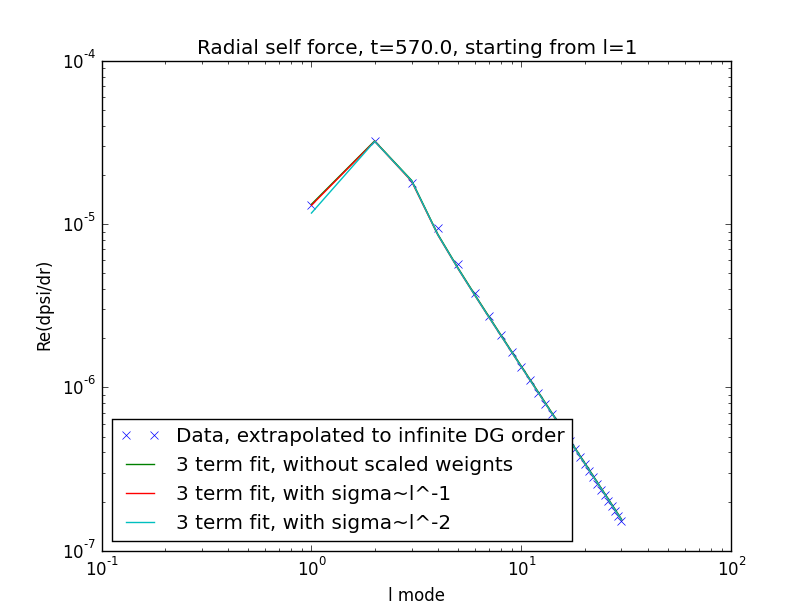
\includegraphics{fiterrscalecorrect3term570l1}
  \caption{t=570, l=1, three term fit with two different power law scales for weights in comparison to unscaled weights ($\sigma=1$).}
\end{figure}


\begin{figure}
  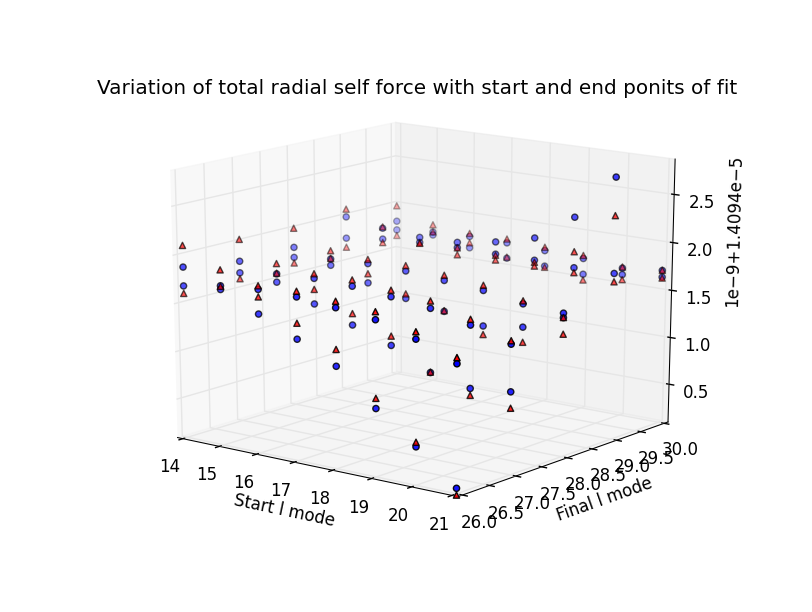
\includegraphics{3Dscatterwithwithoutsigmalminlmax}
  \caption{The difference between the triangles and the circles shows that the difference in the total radial self force between the presence of a $\sigma\sim l^{-2}$ weight and no weight is unimportant compared to the difference in the total radial self force between various start and end points of the l-mode fit.}
\end{figure}

\begin{figure}
  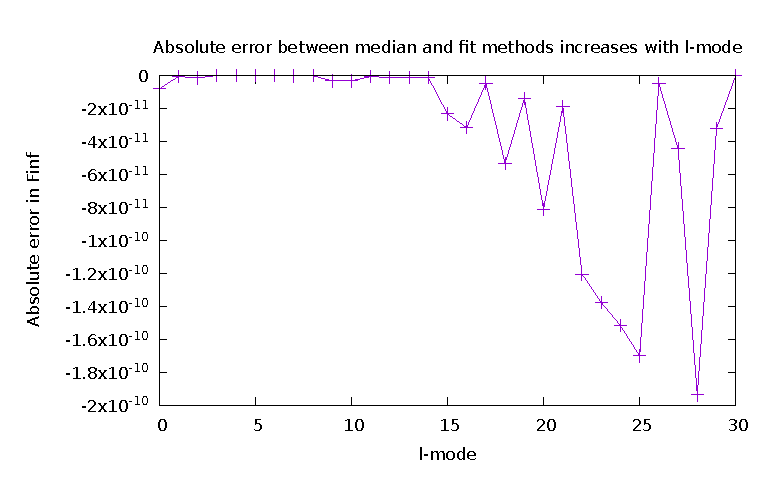
\includegraphics{absErrorIncreaseslmode}
  \caption{Absolute error between fit and median techniques increases with l-mode, explaining why the difference between weight and no weight fit techniques is unimportant.}
\end{figure}

Absolute error increases as l. 


\section{ToDO}
He also wants convergence plots of the fit data versus the median data for some bad times. I also want a plot that shows the raw data before the subtraction of the offset for some time. Modify code to use saved raw data.
